\begin{figure*}{
  \centering
  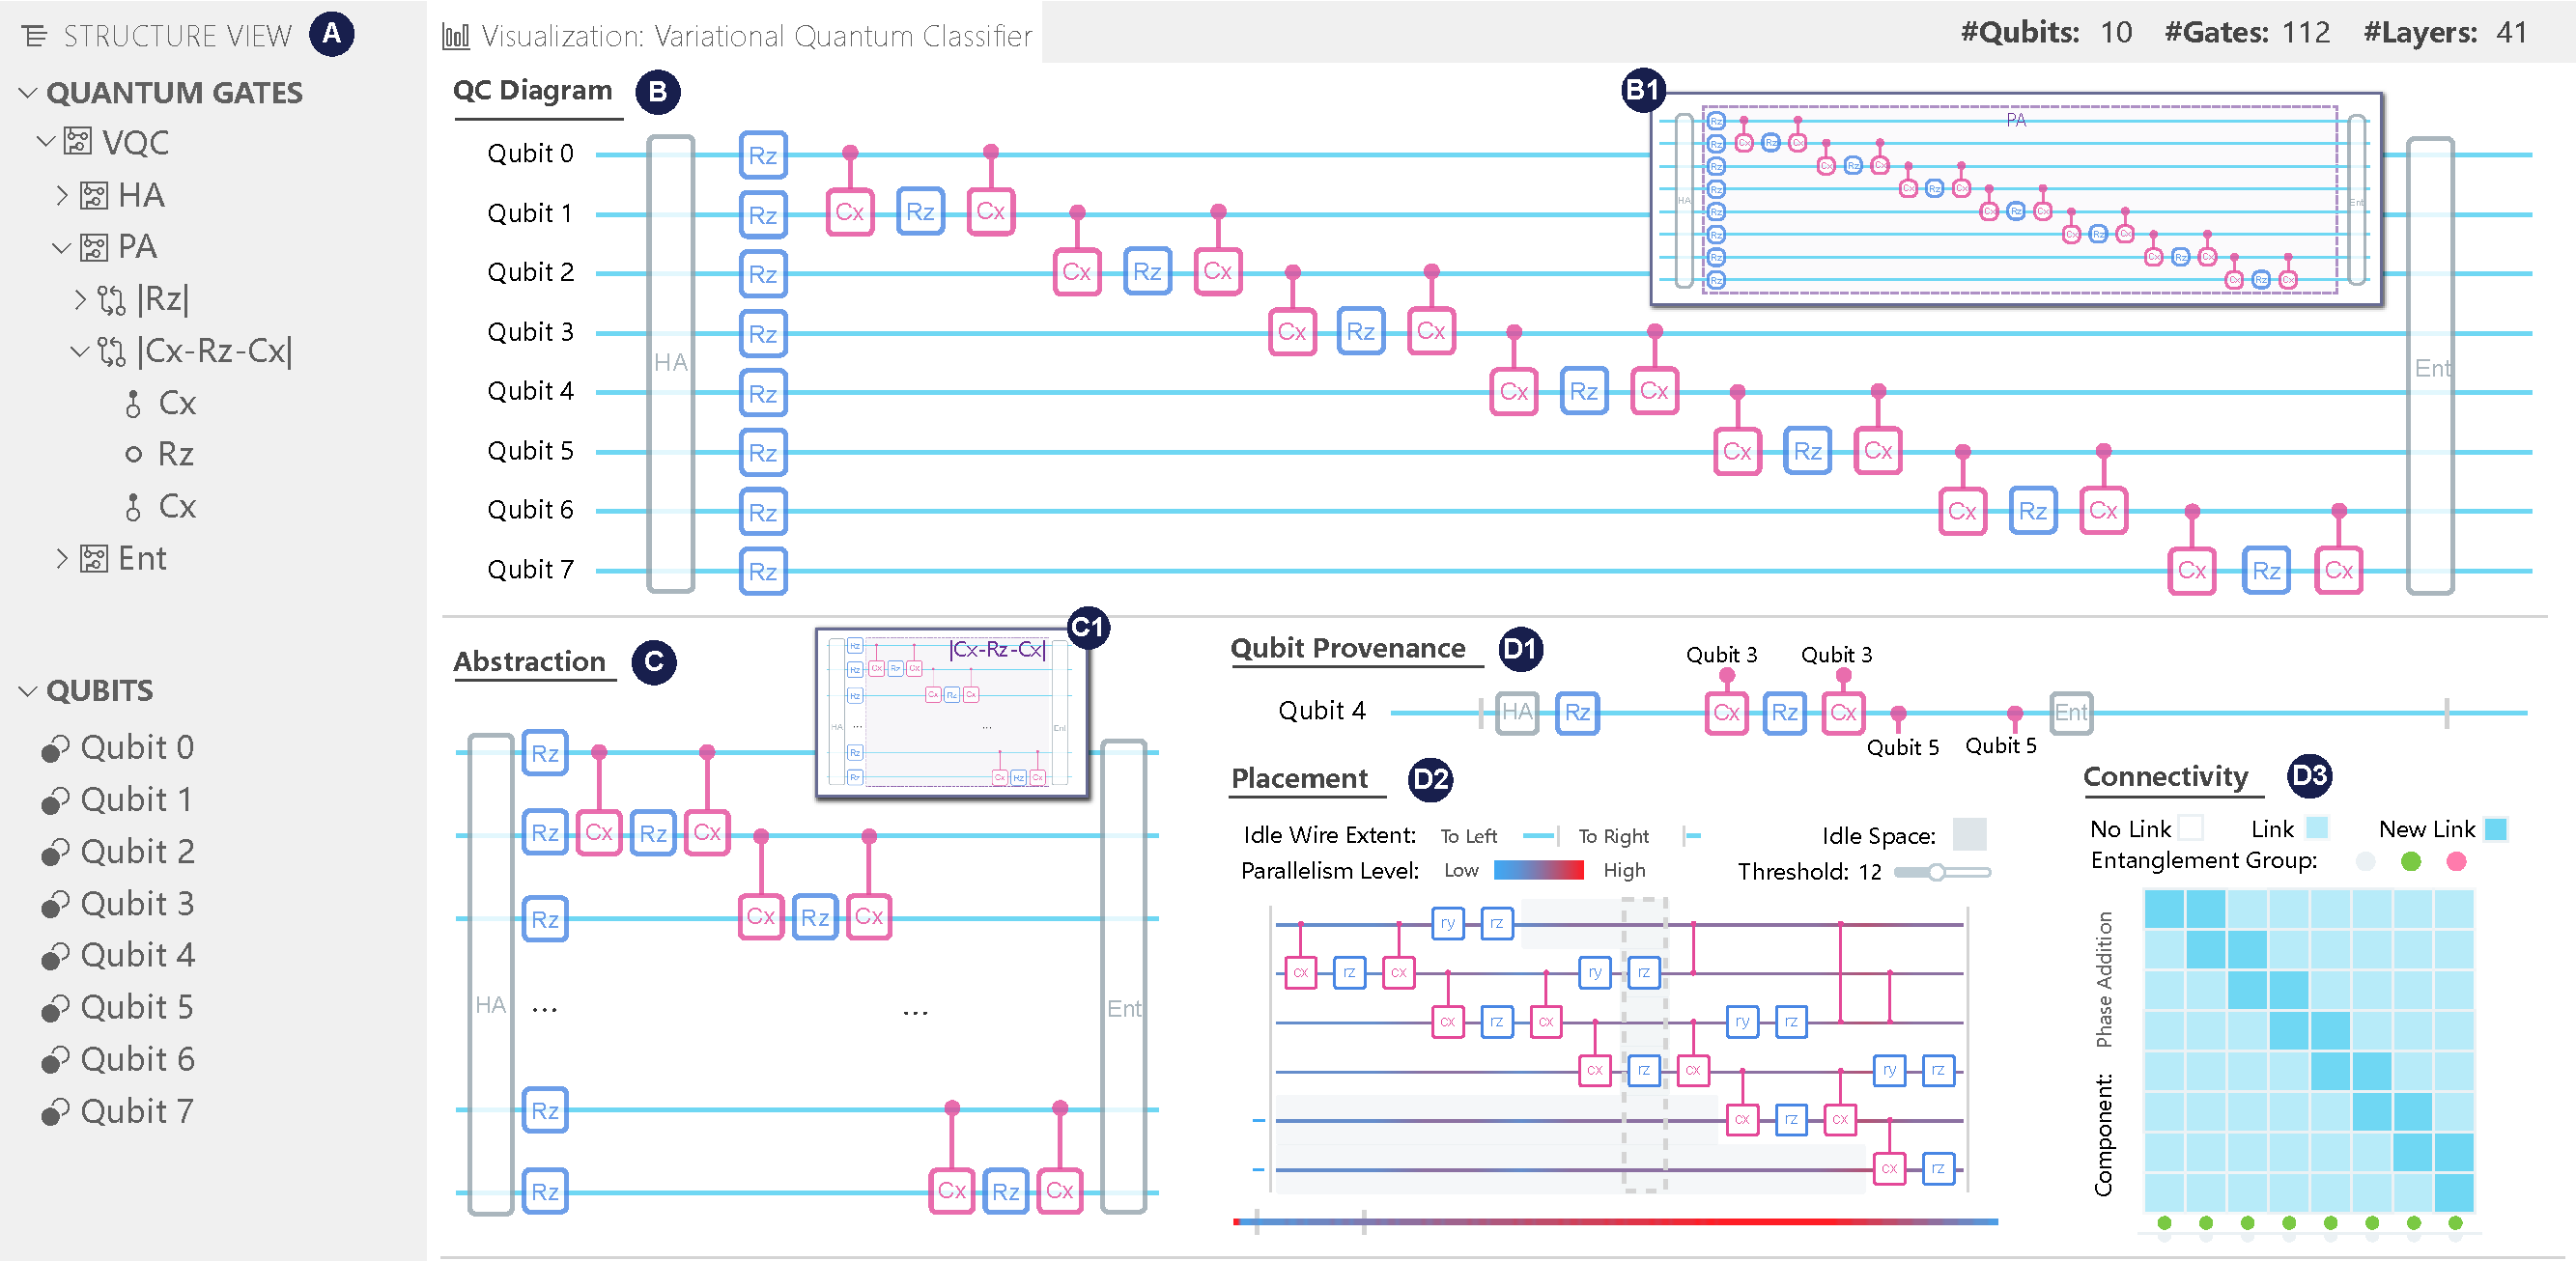
\includegraphics[width=\linewidth]{system-ui}
  \caption{%
    The system interface of {\tname}.
    The Structure View (A) presents the construction of a quantum circuit in a tree diagram including primitive gates, component gates, and repetitive patterns. 
    The Component View (B) provides a flexibly-organized circuit diagram with grouped component gates.
    The Abstraction View (C) shows a further simplified circuit diagram according to visual abstractions of repetitive patterns.
    Three Context Views reveal contextual information in the circuit, including qubit provenance (D1), gate placement (D2), and connectivity (D3).
    %
  }
  \label{fig:system-ui}
}
\end{figure*}


\section{Quantivine: User Interface}
\label{sec:system}
In this section, we introduce the user interface design of {\tname}, which is motivated by our proposed visualization approach,
including the interface design (\cref{sec:system:interface}) and the interaction design (\cref{sec:system:interaction}).
% The system will be used as a technical probe for the usage scenarios (\cref{sec:scenario}) and the user evaluation (\cref{sec:eval}).
\label{sec:ui-design}

% \subsection{System Design}
% The structure view outlines the circuits and acts a part of controller in the system.
% Users use it to navigate in massive quantum circuits, as well as control the organization and the level of details of circuit diagrams.
% Consequently, the visualization view presents the customized visual representations generated by our visualization approach.

\subsection{Interface Design}
\label{sec:system:interface}An overview of the {\tname} interface is shown in \cref{fig:system-ui}, which consists of views (A-D) that present the results of our visualization approach.
{\tname} visualizes the quantum circuit from four aspects:

\begin{itemize}[leftmargin=10pt, noitemsep]
  \item \emph{Structure:}
    The \emph{Structure View} (\cref{fig:system-ui}-A) presents the semantic structure of the quantum circuit as a tree diagram.
    This view serves to provide an overview of the circuit ({R1}) and allows for flexible customization of the circuit visualizations ({R4}). 
    % This view aims to give an overview of the circuit, and serves as a controller to enable flexible customization on the circuit visualizations.
    The tree structure corresponds to the semantic tree extracted from the source code (\cref{sec:code}).
    The branches of the tree outline the hierarchical components and repetitive patterns of the circuit.
    % The components and repetitive patterns of the circuit are hierarchically outlined in the branches of the tree.
    Three interactions based on this view are also designed and further elaborated in \cref{sec:system:interaction}.
    % The components and patterns of the circuit are organized according to collapsible state of each tree item in the structure view.
    % \yezi{User interactions:}
    % We designed three types of interaction, thus enabling users to obtain a better understanding of the circuit and explore it more flexibly (\textbf{R4}).

  \item \emph{Components:}
    The \emph{Component View} (\cref{fig:system-ui}-B) presents a quantum circuit diagram in a generalized form where subsets of quantum gates are aggregated into components.
    This view aims to provide a high-level abstraction of the circuit structure, emphasizing the modularity and reusability of the components ({R1}).
    The components are grouped and arranged based on their execution time and semantics, as extracted from the source code (\cref{sec:segment}).
    The users can use interactions in the \emph{Structure View}, as detailed in \cref{sec:system:interaction}, to customize the level of detail in this view ({R4}).
    % When users completed the design of quantum algorithm, visualizing the circuit which are presented by hierarchical components can provide the pipeline of the algorithm more explicitly. 
    % The gates revealed in structure view will be displayed directly in this part.
    % \yezi{For example, ...}
    % Meanwhile, it is easier for users to spot redundant gate with the assistance of component visualization. \yezi{(fig?)}

  \item \emph{Abstractions:}
    % The \emph{Abstraction View} (\cref{fig:system-ui}-C) presents a more abstract representation of the quantum circuit, where patterns of gates are represented by corresponding visual abstractions.
    The \emph{Abstraction View} (\cref{fig:system-ui}-C) presents the patterns of quantum gates.
    It aims to provide a global perspective of the circuit, highlighting the repetitive patterns and simplifying the visual representation ({R2}).
    % We found that it is highly required to explore the details of quantum circuit which are composed of repetitive patterns most of time. 
    Even though the \emph{Component View} enables scaling down the circuit diagram to a certain extent, it might still take up a large space due to the numerous repeated patterns.
    Hence, we identify and visually abstract such patterns using our approach outlined in \cref{sec:pattern-abs}.
    The level of detail in this view is consistent with the \emph{Component View}.
    % Therefore, abstraction information extracted from the process of pattern abstraction(\Cref{sec:pattern-abs}) will be leveraged to simplify the circuit.\yezi{(fig+example)}

  \item \emph{Context:}
    The \emph{Context Views} (\cref{fig:system-ui}-D1,D2, and D3) consist of three views.
    The first view, D1, provides a summary of the provenance of a qubit within a limited space.
    % First, the provenance of a qubit is summarized in a limited space as D1.
    The second view, D2, depicts the actual placement of quantum gates while visualizing contextual idling and parallelism information.
    % Second, the actual placement of quantum gates are shown in D2, which is visually augmented by contextual idling and parallelism information.
    % Third, the matrix in D3 shows connectivity and entanglement between qubits.
    The third view, D3, displays the matrix showing the connectivity and entanglement between qubits.
    % giving prominence to implicit contextual information in the quantum circuit.
    These views are designed to uncover implicit contextual information within the quantum circuit ({R3}).
    % \st{, to facilitate the detailed analysis of the quantum circuit}
    Additionally, they are interactive and coordinated with other views for specific analysis needs ({R4}).
    % \st{Detailed explanations of the interactive features can be found in \cref{sec:system:interaction}.}
    % We also provided context-oriented visualization. Hence, users can only focus on the gates they are concerned about.\yezi{(fig+example)}
    
\end{itemize}

\subsection{Interactions}
\label{sec:system:interaction}

We implement two interactions in the \emph{Structure View} to enable users to customize the circuit diagrams ({R4}): \emph{folding} and \emph{highlighting}.
% \begin{itemize}[leftmargin=10pt, noitemsep]
\emph{Folding} allows users to fold/unfold items in the \emph{Structure View}.
Initially, all items in the structure tree are collapsed, providing a high-level summary of the circuit. 
Users can expand the items of interest in the tree to explore specific components in more detail. 
This allows users to obtain a more detailed view of the circuit by expanding more low-level items.
With the \emph{highlighting} operation, when users select a particular tree item in the \emph{Structure View}, the corresponding gate will be highlighted in the circuit diagrams in both the \emph{Component} and \emph{Abstraction Views} (\cref{fig:system-ui}-B1,C1). This reduces the manual effort required to match items between code structure and the quantum circuit, and the hierarchical highlights provide a clear division of complex circuit diagrams.
% \end{itemize}


% Users usually find it tedious to map \yezi{code} to its corresponding gate in the large-scale circuit. Highlighting is provided to address this problem.
% \textbf{Focusing.}
% An issue when exploring the details of \yezi{a} certain component in quantum circuit, is that numerous unrelated gates around might distract users. We solved this challenges by providing focusing, which enables users to only pay attention to the components they are interested in since irrelevant part will \yezi{not be displayed(fig.)}.

To facilitate exploration of context information, we design a series of interactions for the \emph{Context Views} in accordance with {R3}.
Users can select a specific qubit in the structure view to display its provenance (\cref{fig:system-ui}-D1).
Clicking on the gates associated with this qubit enables navigation to its placement within the context.
In the placement view, users can adjust the threshold of parallelism level via a scroll bar.
Clicking on a specific column of gates shows potential adjustment places for current parallel operations.
In terms of connectivity, \emph{Quantivine} allows users to specify a component and highlight its connections and entanglement behaviors for a more comprehensive view of the circuit.


\begin{figure*}[tb]
    \centering
    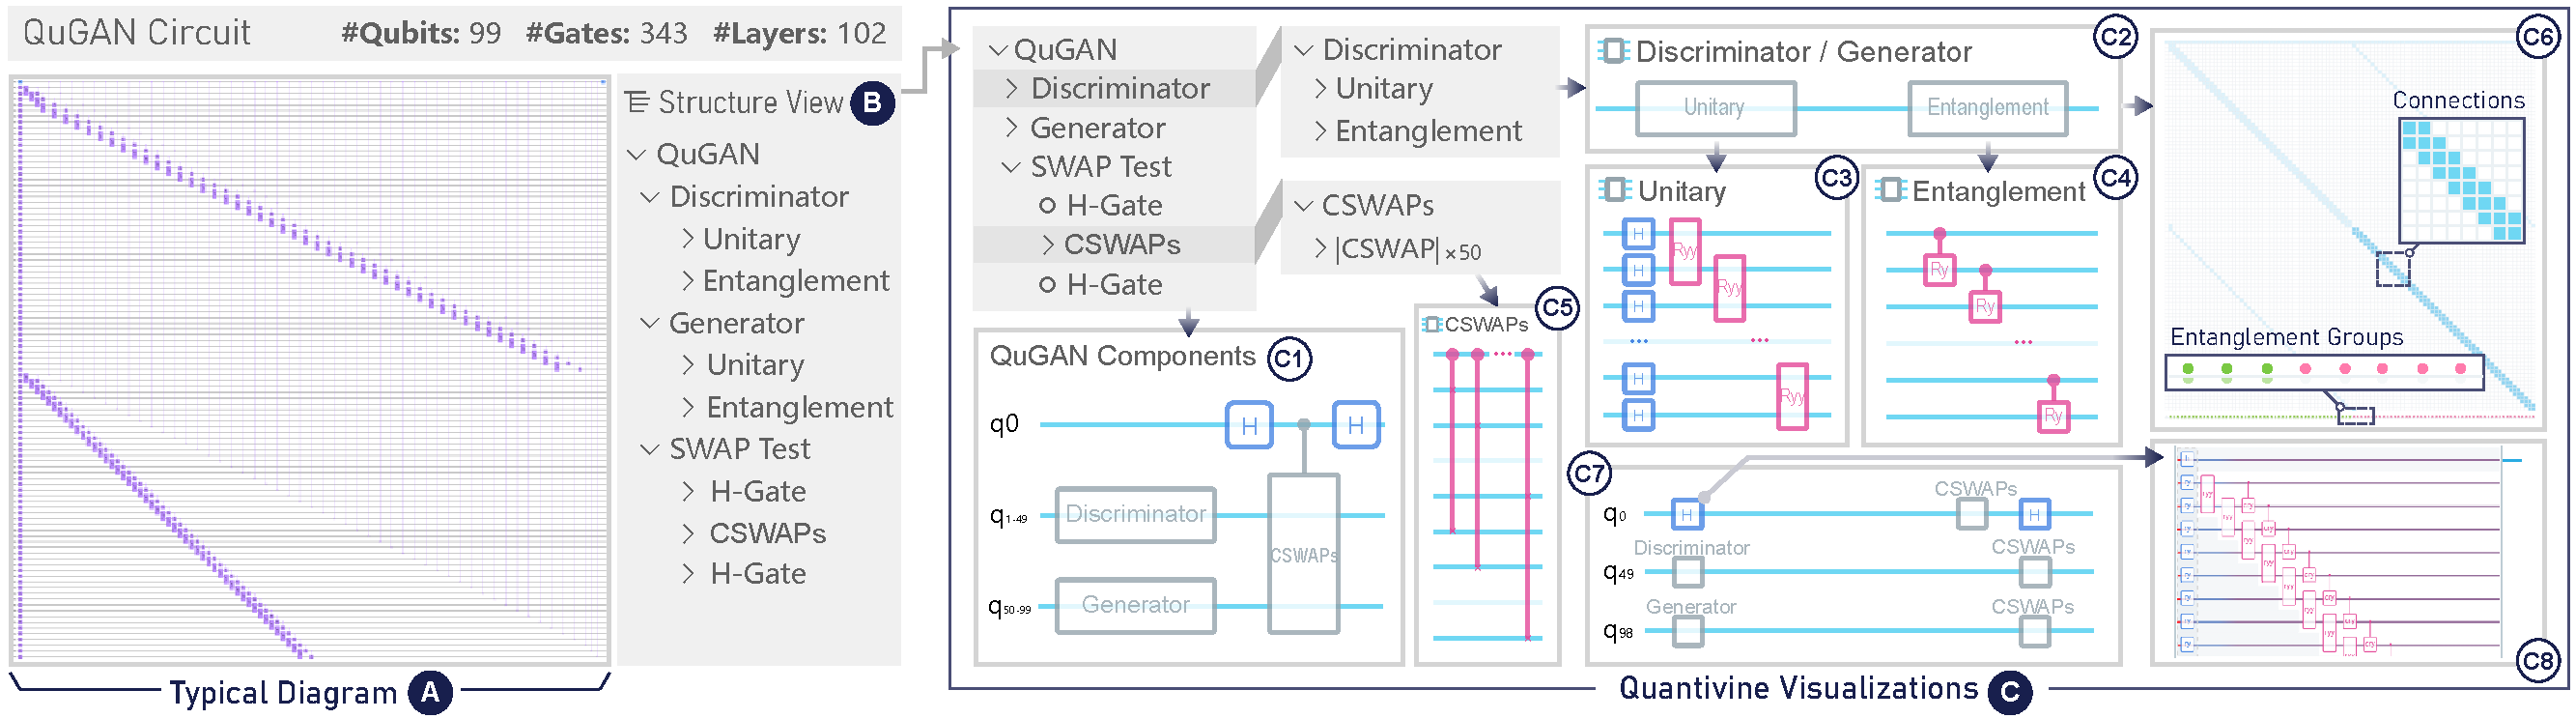
\includegraphics[width=\linewidth]{case-1}
    \caption{%
        {\tname} generates visualizations based on a 99-qubit QuGAN circuit (A).
        The structure view (B) lists the components of QuGAN.
        User interactions results in visualizations from the component view (C1-2), abstraction view (C3-5) and context views (C6-8).
        %
    }
    \label{fig:case-1}
\end{figure*}

\begin{figure*}[b]
  \centering
  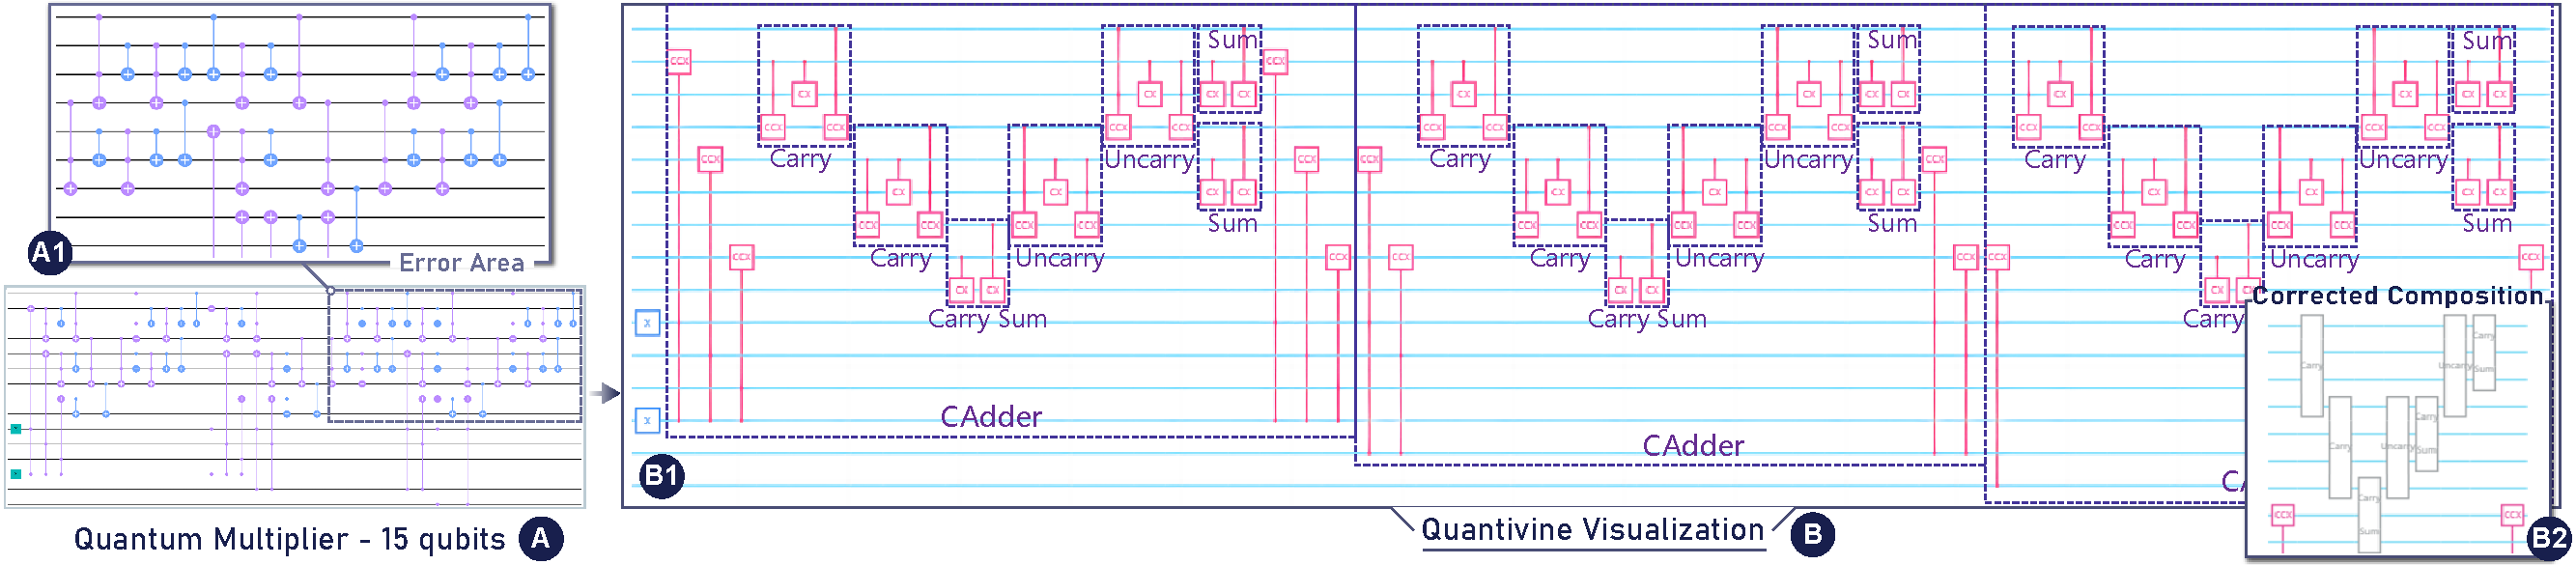
\includegraphics[width=\linewidth]{case-2}
  \caption{%
    {\tname} wrangles a complex and unstructured quantum circuit diagram (A) into a clear and organized visualization (B) that enables users to easily navigate and identify errors in the circuit.
  }
  \label{fig:case-2}
\end{figure*}


% \subsection{Implementation}
% The system is a webview-based editor plugin written in Typescript, HTML, and CSS using the framework \emph{React JS}.
% To facilitates the efficient rendering, the quantum circuit diagrams are rendered using Canvas, while the other visual cues are rendered as SVGs.
% The input source code is processed using separate Python scripts.
% The visualization results of different quantum programs are included in the supplementary materials.

\section{Usage Scenarios}
\label{sec:scenario}
In this section, we demonstrate the effectiveness of \emph{Quantivine} through two usage scenarios with domain experts.
The first scenario (\cref{sec:scenario-1}) shows the exploration of a 99-qubit quantum circuit that implements a quantum neural network model.
The second scenario (\cref{sec:scenario-2}) introduces the workflow of bug identification in a quantum algorithm.

\subsection{Scenario 1 - Visual Analysis of QuGAN}
\label{sec:scenario-1}
Quantum Generative Adversarial Network (QuGAN) is an emerging topic of quantum machine learning\cite{Stein:2021:QuGAN}. 
However, as shown in \mbox{\cref{fig:case-1}-A}, the meaning of gates in a typical 99-qubit circuit diagram of QuGAN is difficult to understand due to a lack of semantic information.

The expert E1 intends to implement QuGAN on a real quantum computer. Thus, he is interested in exploring the functionality of each part of the QuGAN circuit. 
E1 first examines the high-level structure of QuGAN in the \emph{Structure View} (\cref{fig:case-1}-B): the Discriminator, Generator, and SWAP Test.
After collapsing the components, the circuit diagram becomes clearer and easier to comprehend (\cref{fig:case-1}-C1).
E1 then visualizes the detailed structure of the circuit.
By expanding the Discriminator and Generator components, E1 discovers that they both consist of a Unitary component and an Entanglement component (\cref{fig:case-1}-C2).
Upon further expansion, E1 finds that these components include quantum gates that show repeated patterns.
To confirm the role of these components, E1 employs the connectivity matrix to analyze the connections between different qubits.
As such, E1 leverages the \emph{Abstraction View} to get a concise view of these patterns. In \cref{fig:case-1}-C3, the Unitary component includes a sequence of Ryy gates, connecting qubits in a linear manner. In \cref{fig:case-1}-C4, instead of Ryy gates, the Entanglement component involves linearly-connected CRy gates. E1 says, ``With my knowledge of quantum machine learning, now I understand why the Discriminator and Generator have the same structure. Analogous to classical neural networks, QuGAN trains the parameters of gates to fit the data. In the GAN framework, both the discriminator and generator are neural networks. Thus, their two quantum versions use the same model for simplicity.'' 
To verify this observation, he then highlights the Discriminator, Generator, and SWAP Test components in the matrix view~(\Cref{fig:case-1}-C6), which shows
that the qubits of the Generator component are fully connected. ``This is designed to utilize the unique entanglement property of quantum physics to improve the model complexity, which further improves the prediction accuracy,'' said E1. He also notices that the SWAP Test component entangles all the qubits at the end, as shown in \cref{fig:case-1}-C5, which sends the predictions from the Generator to the Discriminator.

After grasping the detailed structure of the circuit, E1 decides to collapse the details, keeping an overview of it as shown in \cref{fig:case-1}-C1.
He then proceeds to analyze the circuit in terms of the arrangement of qubits and quantum gates.
He first selects q0, and the qubit provenance view shows that it passes through an H-gate, a CSWAPs component, and another H-gate (\cref{fig:case-1}-C7).
This provenance demonstrates that q0 is acting as a control qubit in the SWAP test.
However, via \cref{fig:case-1}-C8, E1 identifies a suboptimal placement of the first H-gate and the CSWAPs component, as there is significant idle time between these operations, which might introduce noise when executed on a quantum computer.
Therefore, he clicks on these two gates to check if it is possible to adjust their placement.
In the placement view, the visual cues show that there is a space for the H-gate to move backwards (\cref{fig:case-1}-C8).
The color of the qubit wire indicates a possible location on the left of the next gate with a low parallelism level, which is suitable for replacing the H-gate. 

% After optimizing the placement of the gates, E1 successfully reduces the total idling time of the circuit.
% With the help of {\tname}, E1 was able to efficiently explore and analyze the large QuGAN circuit diagram, demonstrating the practicality of the system in quantum circuit analysis.

\subsection{Scenario 2 - Bug Detection of Quantum Multiplier}
\label{sec:scenario-2}
The complexity of quantum circuits makes it difficult to detect bugs at the circuit level.
The quantum multiplier, which is designed to calculate the product of two numbers stored in qubits, is a prime example of this complexity.
Even a small-scale quantum multiplier has an intricate structure that is arduous to grasp (\cref{fig:case-2}-A).
% ,making it a challenging task for both novice and expert users to implement a scalable quantum multiplier.

The expert E2 is tasked with detecting bugs in a 15-qubit quantum multiplier circuit, where the bugs are hidden within a cluttered area of the circuit diagram (\cref{fig:case-2}-A1).
To accomplish this, he employs {\tname} to visualize and explore the construction of the circuit.
E2 starts by collapsing all sub-components to obtain an overview of the circuit.
After confirming the high-level structure of the circuit is correct in the \emph{Component View}, he guesses that the bugs are hidden within more detailed structures.
Thus, he drills down by expanding all components.
% Due to benefits of our layout strategy, the fully expanded circuit become though lengthy, it kept an ordered and semantic layout.
Despite the circuit becoming lengthy when fully expanded, our layout strategy ensures an organized and semantically meaningful layout~(\cref{fig:case-2}-B1).
% E2 highlights the components from high-level to low-level and {\tname} provides a more clear and structured representation of the circuit, as shown in \cref{fig:case-2}-B1. 
% He continues to highlight the components from high-level to low-level in order, \emph{Quantivine} provides a clear and structured representation of the circuit, as shwon in \cref{fig:case-2}-B1.
In this view, he notices that the composition of the UnCarry and Sum components in the Adder is incorrect, which should be composed as shown in \cref{fig:case-2}-B2.
Guided by the structured view and visual cues of the circuit diagram, E2 quickly locates the bugs in the underlying code of the circuit and effectively fixes them.
% He found that the multiplier had a multi-level and complicated structure from the \emph{Structure View} (\cref{fig:case-2}-A1).
% He thus collapsed most sub-components to examine a high-level structure of the circuit (\cref{fig:case-2}-A2).
% The \emph{Component View} depicted that a series of controlled adders (CAdder) forms a multiplier.
% Next, E2 expanded CAdders to explore their constructions.
% \Cref{fig:case-2}-A3 illustrates that the CAdder component was controlled by two groups of CCX-gate alongside,
% and its core component, Adder, was comprised of Carry, Sum, and UnCarry components.
% Then, E2 expanded these components to see their internal structure and composition pattern.
% Due to benefits of our layout strategy, the fully expanded circuit become though lengthy, it kept an ordered and semantic layout.
% E2 applied highlighting interactions to clarify the border between various components.
% The overall structure of quantum multiplier was clearly represented as shown in \cref{fig:case-2}-A4.
% E2 also compared the experience of examining the circuit diagram generated by Qiskit (\cref{fig:case-2}-B).
% He tried to build connections between the programming code and the diagram in his mind,
% to comprehend the meanings of circuit structure, but found it required heavy mental load and error-prone.
% In contrast, the experience of using \emph{Quantivine} is easy and efficient.

% In summary, a series of resulting visualizations provide a concise and hierarchical representation of the structure of the quantum multiplier, which is beneficial for both novice and expert users.
% The use of \emph{Quantivine} for circuit representation enables a faster and more efficient understanding of complex quantum circuits, which is crucial for the development of scalable quantum applications.
% \emph{This process of converting specifications to program code is unintuitive and tricky.}\cite{Huang:2019:SAVA}


% \subsubsection{Finding Bugs}

% \textbf{Incorrect operations and transformations.} \emph{These possible bugs include \textcolor{blue}{indexing errors} in the two-dimensional loop, bit shifting errors, endian confusion, and mistakes in rotation angles.}

% \textbf{Incorrect composition of operations.}

% \textbf{Incorrect entanglement.}


% \subsubsection{Optimization}
% Optimization.


